\documentclass{article}

\usepackage{xecjk}
\usepackage{algorithm}
\usepackage{algorithmic}
\usepackage{geometry}
\usepackage{enumerate}
\usepackage{amssymb}
\usepackage{amsmath}
\usepackage{graphics}
\usepackage{graphicx}

\geometry{a4paper, scale = 0.8}

\begin{document}
    \title{Puzzle Bobble实验报告}
    \author{name: \underline{邱圆辉} \qquad student number: \underline{2017013591}}
    \date{}
    \maketitle

    \section{操作说明}
        \subsection{主界面}
        \begin{figure}[H]
            \centering
            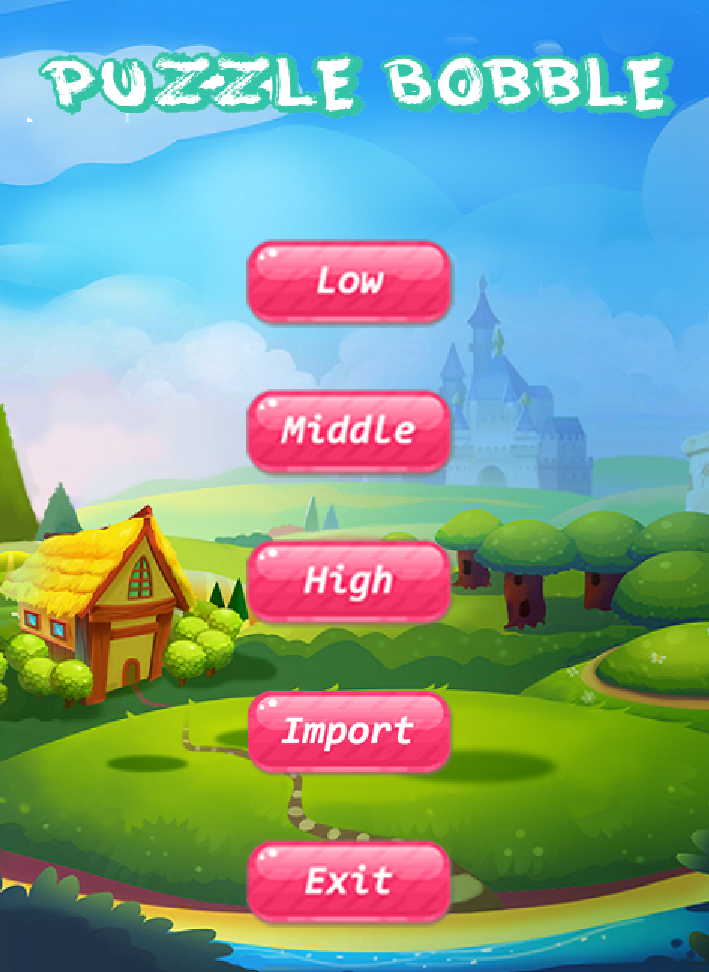
\includegraphics[scale=0.5]{mainScene.png}
        \end{figure}
        \begin{enumerate}
            \item \textbf{low按钮}\\
            点击进入低难度关卡。(初始三排泡泡,包含三种不同颜色)
            \item \textbf{middle按钮}\\
            点击进入中难度关卡。(初始四排泡泡,包含四种不同颜色)
            \item \textbf{high按钮}\\
            点击进入高难度关卡。(初始五排泡泡,包含五种不同颜色)
            \item \textbf{import按钮}\\
            点击跳出选择配置文件的窗口,选择完毕后会游戏会加载配置文件中描述的配置。
            \item \textbf{exit按钮}\\
            点击退出游戏。
        \end{enumerate}

        \subsection{游戏界面}
        \begin{figure}[H]
            \centering
            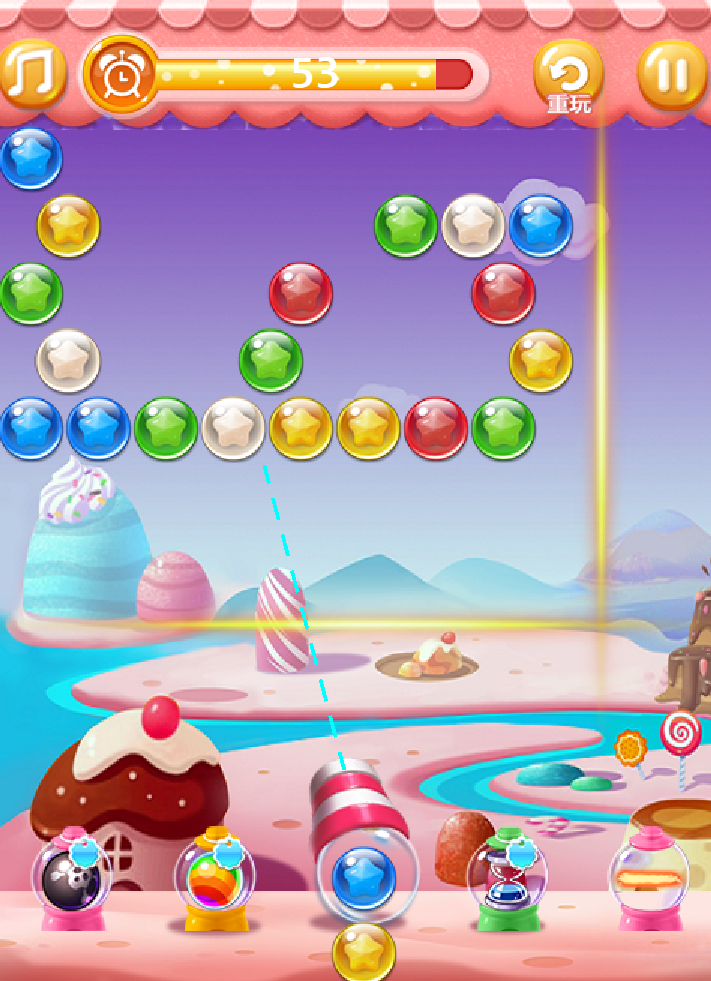
\includegraphics[scale=0.5]{playScene.png}
        \end{figure}
        \begin{enumerate}
            \item \textbf{静音按钮(左上角)}\\
            点击可设置游戏为静音,再次点击可恢复音乐和音效。
            \item \textbf{暂停按钮(右上角)}\\
            点击暂停游戏,再次点击继续游戏。
            \item \textbf{重玩按钮(右上角)}\\
            点击返回至难度选择界面。
            \item \textbf{背景图片(中央)}\\
            点击背景图片,即泡泡墙所处位置即可发射泡泡。
            \item \textbf{时间条(正上方)}\\
            显示当前剩余游戏时间。
            \item \textbf{发射器(正下方)}\\
            发射器中的泡泡为当前即将发射的泡泡,发射器下方为下一个泡泡。
            位于发射器左右两边的四个道具从左至右分别为:
            \item \textbf{生命线(发射器上方黄色线)}\\
            标示游戏的生命线,若泡泡墙深度超过此线则游戏失败。
            \item \textbf{边界线(右方黄色线)}\\
            游戏默认最大泡泡列数为10,边界线即为窗口右边界。
            若配置文件中描述的最大列数小于10,则在右方会有一条黄色边界线,泡泡到达此边界后会按反射定律反弹。
            
            \begin{itemize}
                \item \textbf{炸弹} \\
                 点击后当前泡泡会被替换为炸弹,炸弹到达泡泡墙后会消除与其相邻的所有泡泡。
                \item \textbf{彩虹} \\
                点击后当前泡泡会被替换为彩虹,彩虹到达泡泡墙后会随机变换颜色为与其相邻泡泡中的一种。
                \item \textbf{沙漏} \\
                点击后当前游戏时间增加10秒,但是不会超过60秒。
                \item \textbf{激光} \\
                点击后泡泡墙中除第一行泡泡外,其余所有泡泡均下落并消失。
            \end{itemize}
        \end{enumerate}

        \section{游戏结束界面}
            \subsection{胜利界面}
            \begin{figure}[H]
                \centering
                
\includegraphics[scale=0.5]{win.png}
            \end{figure}
            游戏胜利场景。(在规定时间内将泡泡消完或时间耗尽后剩余泡泡小于等于5)点击返回首页按钮可返回至关卡选择界面。

            \subsection{失败界面}
            \begin{figure}[H]
                \centering
                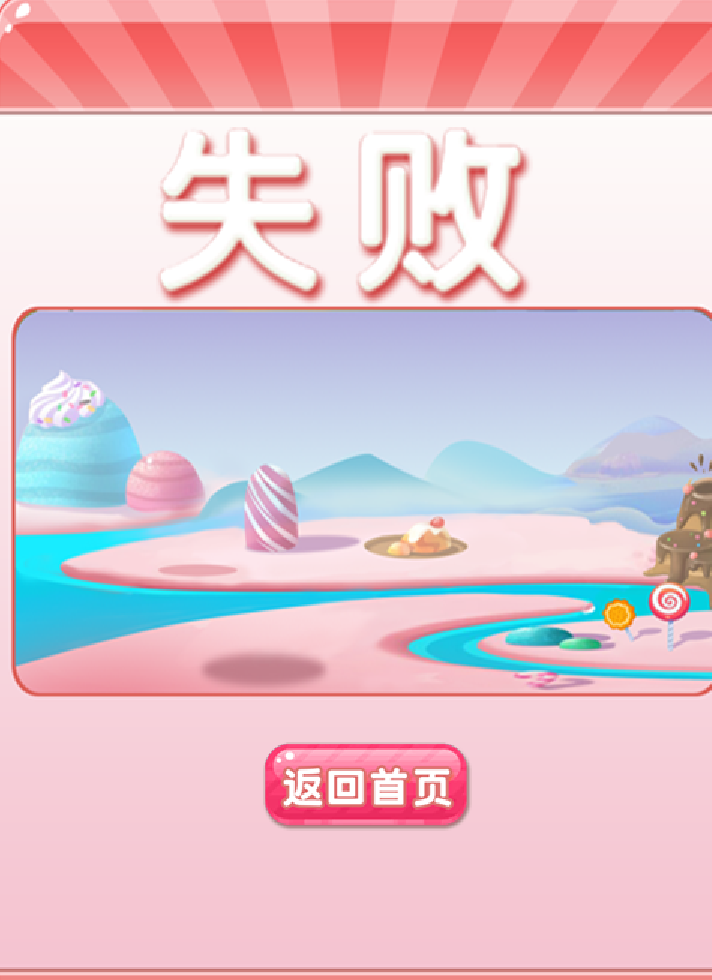
\includegraphics[scale=0.5]{fail.png}
            \end{figure}
            游戏失败场景。(时间耗尽后剩余泡泡大于5或泡泡墙深度超过生命线)点击返回首页按钮可返回至关卡选择界面。

    \section{说明}
    \begin{enumerate}
        \item 本次游戏架构采用了MFC设计模式:
        绘图由$MyContentPanel$类控制,并下发给不同场景类执行;
        事件响应由$MouseEventHandler$类控制,并下发给$Control$类执行;
        数据由$PlayScene$类负责掌管并更新。
        \item 程序默认最大泡泡列数为10,最大泡泡行数为9,最大游戏时间为60s,最大泡泡颜色种类为5,因此配置文件中请不要输入大于这些的数值。
        \item 由于时间关系,程序在读取配置文件时未进行错误处理,因此测试时请严格按照$example.txt$中的格式进行输入,且不要输入错误参数。(即泡泡矩阵的行数大于最大行数或泡泡矩阵的列数不等于最大列数等)
        \item 程序实现了所有基本功能和提高功能,测试时按照如上说明测试即可。
    \end{enumerate}
    
\end{document}